\documentclass[11pt,preprint]{elsarticle}

\usepackage{lmodern}
%%%% My spacing
\usepackage{setspace}
\setstretch{1.2}
\DeclareMathSizes{12}{14}{10}{10}

% Wrap around which gives all figures included the [H] command, or places it "here". This can be tedious to code in Rmarkdown.
\usepackage{float}
\let\origfigure\figure
\let\endorigfigure\endfigure
\renewenvironment{figure}[1][2] {
    \expandafter\origfigure\expandafter[H]
} {
    \endorigfigure
}

\let\origtable\table
\let\endorigtable\endtable
\renewenvironment{table}[1][2] {
    \expandafter\origtable\expandafter[H]
} {
    \endorigtable
}


\usepackage{ifxetex,ifluatex}
\usepackage{fixltx2e} % provides \textsubscript
\ifnum 0\ifxetex 1\fi\ifluatex 1\fi=0 % if pdftex
  \usepackage[T1]{fontenc}
  \usepackage[utf8]{inputenc}
\else % if luatex or xelatex
  \ifxetex
    \usepackage{mathspec}
    \usepackage{xltxtra,xunicode}
  \else
    \usepackage{fontspec}
  \fi
  \defaultfontfeatures{Mapping=tex-text,Scale=MatchLowercase}
  \newcommand{\euro}{€}
\fi

\usepackage{amssymb, amsmath, amsthm, amsfonts}

\def\bibsection{\section*{References}} %%% Make "References" appear before bibliography


\usepackage[numbers]{natbib}

\usepackage{longtable}
\usepackage[margin=2.3cm,bottom=2cm,top=2.5cm, includefoot]{geometry}
\usepackage{fancyhdr}
\usepackage[bottom, hang, flushmargin]{footmisc}
\usepackage{graphicx}
\numberwithin{equation}{section}
\numberwithin{figure}{section}
\numberwithin{table}{section}
\setlength{\parindent}{0cm}
\setlength{\parskip}{1.3ex plus 0.5ex minus 0.3ex}
\usepackage{textcomp}
\renewcommand{\headrulewidth}{0.2pt}
\renewcommand{\footrulewidth}{0.3pt}

\usepackage{array}
\newcolumntype{x}[1]{>{\centering\arraybackslash\hspace{0pt}}p{#1}}

%%%%  Remove the "preprint submitted to" part. Don't worry about this either, it just looks better without it:
\makeatletter
\def\ps@pprintTitle{%
  \let\@oddhead\@empty
  \let\@evenhead\@empty
  \let\@oddfoot\@empty
  \let\@evenfoot\@oddfoot
}
\makeatother

 \def\tightlist{} % This allows for subbullets!

\usepackage{hyperref}
\hypersetup{breaklinks=true,
            bookmarks=true,
            colorlinks=true,
            citecolor=blue,
            urlcolor=blue,
            linkcolor=blue,
            pdfborder={0 0 0}}


% The following packages allow huxtable to work:
\usepackage{siunitx}
\usepackage{multirow}
\usepackage{hhline}
\usepackage{calc}
\usepackage{tabularx}
\usepackage{booktabs}
\usepackage{caption}


\newenvironment{columns}[1][]{}{}

\newenvironment{column}[1]{\begin{minipage}{#1}\ignorespaces}{%
\end{minipage}
\ifhmode\unskip\fi
\aftergroup\useignorespacesandallpars}

\def\useignorespacesandallpars#1\ignorespaces\fi{%
#1\fi\ignorespacesandallpars}

\makeatletter
\def\ignorespacesandallpars{%
  \@ifnextchar\par
    {\expandafter\ignorespacesandallpars\@gobble}%
    {}%
}
\makeatother


% definitions for citeproc citations
\NewDocumentCommand\citeproctext{}{}
\NewDocumentCommand\citeproc{mm}{%
\href{\#cite.\detokenize{#1}}{#2}\nocite{#1}}

\makeatletter
% allow citations to break across lines
\let\@cite@ofmt\@firstofone
% avoid brackets around text for \cite:
\def\@biblabel#1{}
\def\@cite#1#2{{#1\if@tempswa , #2\fi}}
\makeatother
\newlength{\cslhangindent}
\setlength{\cslhangindent}{1.5em}
\newlength{\csllabelwidth}
\setlength{\csllabelwidth}{3em}
\newenvironment{CSLReferences}[2] % #1 hanging-indent, #2 entry-spacing
{\begin{list}{}{%
	\setlength{\itemindent}{0pt}
	\setlength{\leftmargin}{0pt}
	\setlength{\parsep}{0pt}
	% turn on hanging indent if param 1 is 1
	\ifodd #1
	\setlength{\leftmargin}{\cslhangindent}
	\setlength{\itemindent}{-1\cslhangindent}
	\fi
	% set entry spacing
	\setlength{\itemsep}{#2\baselineskip}}}
{\end{list}}

\usepackage{calc}
\newcommand{\CSLBlock}[1]{\hfill\break\parbox[t]{\linewidth}{\strut\ignorespaces#1\strut}}
\newcommand{\CSLLeftMargin}[1]{\parbox[t]{\csllabelwidth}{\strut#1\strut}}
\newcommand{\CSLRightInline}[1]{\parbox[t]{\linewidth - \csllabelwidth}{\strut#1\strut}}
\newcommand{\CSLIndent}[1]{\hspace{\cslhangindent}#1}


\urlstyle{same}  % don't use monospace font for urls
\setlength{\parindent}{0pt}
\setlength{\parskip}{6pt plus 2pt minus 1pt}
\setlength{\emergencystretch}{3em}  % prevent overfull lines
\setcounter{secnumdepth}{5}

%%% Use protect on footnotes to avoid problems with footnotes in titles
\let\rmarkdownfootnote\footnote%
\def\footnote{\protect\rmarkdownfootnote}
\IfFileExists{upquote.sty}{\usepackage{upquote}}{}

%%% Include extra packages specified by user
\usepackage{graphicx}
\providecommand{\pandocbounded}[1]{#1}

%%% Hard setting column skips for reports - this ensures greater consistency and control over the length settings in the document.
%% page layout
%% paragraphs
\setlength{\baselineskip}{12pt plus 0pt minus 0pt}
\setlength{\parskip}{12pt plus 0pt minus 0pt}
\setlength{\parindent}{0pt plus 0pt minus 0pt}
%% floats
\setlength{\floatsep}{12pt plus 0 pt minus 0pt}
\setlength{\textfloatsep}{20pt plus 0pt minus 0pt}
\setlength{\intextsep}{14pt plus 0pt minus 0pt}
\setlength{\dbltextfloatsep}{20pt plus 0pt minus 0pt}
\setlength{\dblfloatsep}{14pt plus 0pt minus 0pt}
%% maths
\setlength{\abovedisplayskip}{12pt plus 0pt minus 0pt}
\setlength{\belowdisplayskip}{12pt plus 0pt minus 0pt}
%% lists
\setlength{\topsep}{10pt plus 0pt minus 0pt}
\setlength{\partopsep}{3pt plus 0pt minus 0pt}
\setlength{\itemsep}{5pt plus 0pt minus 0pt}
\setlength{\labelsep}{8mm plus 0mm minus 0mm}
\setlength{\parsep}{\the\parskip}
\setlength{\listparindent}{\the\parindent}
%% verbatim
\setlength{\fboxsep}{5pt plus 0pt minus 0pt}



\begin{document}



\begin{frontmatter}  %

\title{Loans and Credit: Testing the Institute's Beliefs}

% Set to FALSE if wanting to remove title (for submission)




\author[Add1]{22761926}
\ead{22761926@sun.ac.za}





\address[Add1]{Stellenbosch University}

\cortext[cor]{Corresponding author: 22761926}

\begin{abstract}
\small{
This report analyses Lending Club loan data to test three beliefs held
by a Credit Institute, and to answer the Director's questions on default
risk drivers, debt-to-income thresholds, and state-level differences.
}
\end{abstract}

\vspace{1cm}





\vspace{0.5cm}

\end{frontmatter}

\setcounter{footnote}{0}



%________________________
% Header and Footers
%%%%%%%%%%%%%%%%%%%%%%%%%%%%%%%%%
\pagestyle{fancy}
\chead{}
\rhead{}
\lfoot{}
\rfoot{\footnotesize Page \thepage}
\lhead{}
%\rfoot{\footnotesize Page \thepage } % "e.g. Page 2"
\cfoot{}

%\setlength\headheight{30pt}
%%%%%%%%%%%%%%%%%%%%%%%%%%%%%%%%%
%________________________

\headsep 35pt % So that header does not go over title




\section{Overview}\label{overview}

This report analyses Lending Club loan data to test three beliefs held
by the Credit Institute, and to answer the Director's broader questions
on default risk.

A loan's outcome was classified as Fully Paid or Charged Off where
resolved. Current, Late and Grace Period loans were excluded from
default rate calculations, since their final outcome is not yet known.
Across 383,202 resolved loans, the overall default rate is 22.5\%, which
serves as a baseline for comparison throughout this report.

\section{Testing the Director's First Belief: Home Ownership and
Employment
Length}\label{testing-the-directors-first-belief-home-ownership-and-employment-length}

The Director's institute believes home owners and people employed 10+
years have lower default rates on short-term loans.

\pandocbounded{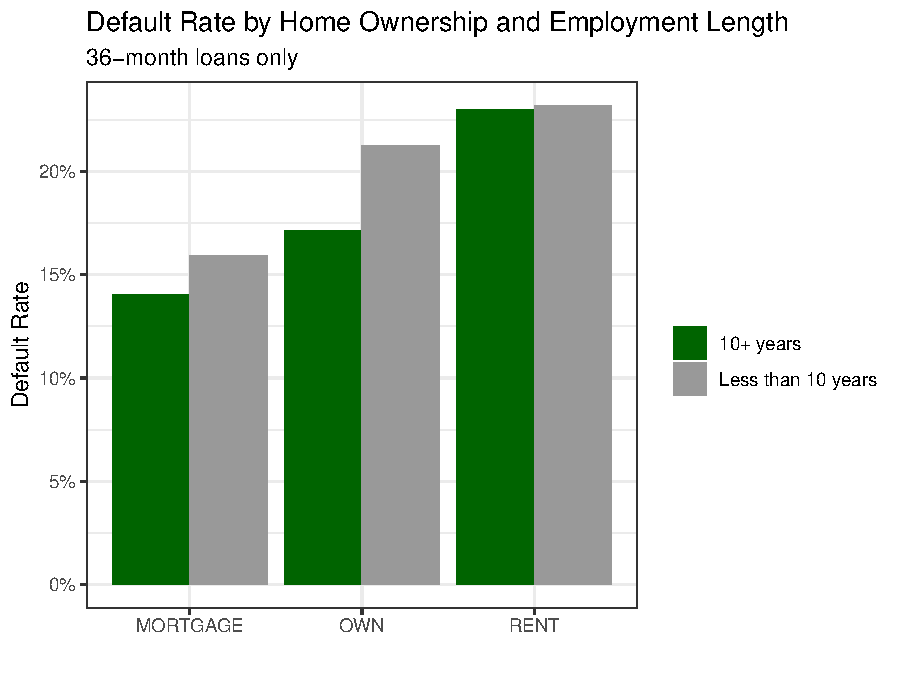
\includegraphics[keepaspectratio]{Question_3_files/figure-latex/unnamed-chunk-1-1.pdf}}

\begin{itemize}
\tightlist
\item
  Mortgage holders default least, at between 14.1\% and 15.9\%.
  Homeowners without a mortgage follow at 17.1\% to 21.3\%. Renters
  default most, at around 23\%.
\item
  Borrowers employed 10+ years default noticeably less than those with
  shorter employment histories, within both the mortgage and homeowner
  categories.
\item
  Employment length makes little difference for renters. Both groups
  default at a similarly high rate. Housing status appears to be the
  stronger signal in this case.
\item
  The Director's belief is well supported by the data, at least for
  short-term, 36-month loans.
\end{itemize}

\section{Testing the Director's Second Belief: State-Level Default
Differences}\label{testing-the-directors-second-belief-state-level-default-differences}

The Director's institute believes US States differ significantly in
their culture of defaulting on short-term loans.

\pandocbounded{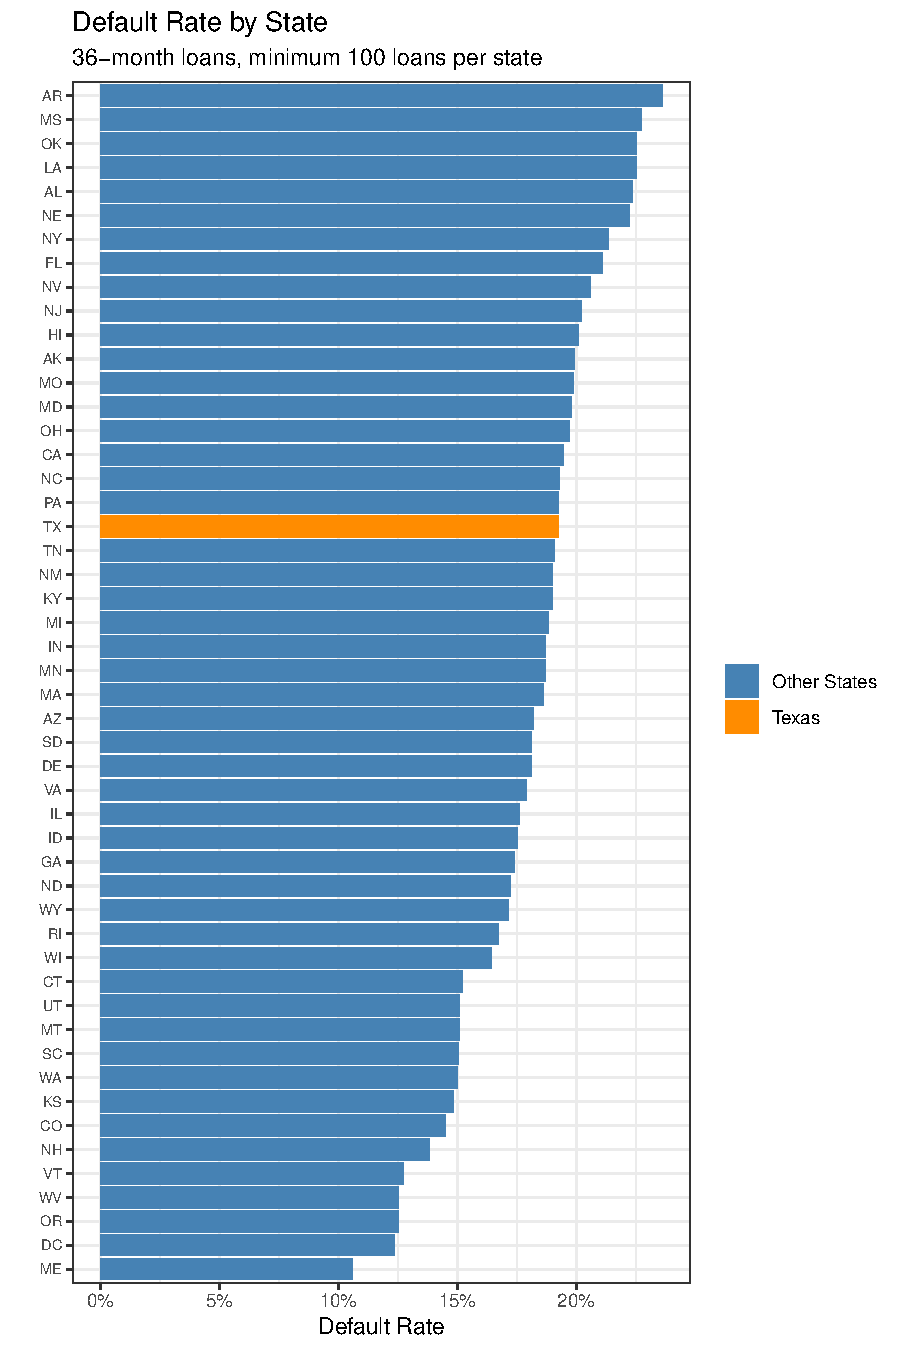
\includegraphics[keepaspectratio]{Question_3_files/figure-latex/unnamed-chunk-2-1.pdf}}

State default rates do genuinely differ. Arkansas sits highest at
23.6\%, while Maine sits lowest at 10.6\%. That gap is more than double,
which supports the Director's belief.

A loose regional pattern emerges too. Several Southern states cluster
near the top of the chart, including Arkansas, Mississippi, Oklahoma,
Louisiana and Alabama. Several Northeastern and mountain states cluster
near the bottom, including Maine, Vermont, West Virginia and Oregon.
This pattern is worth noting, though it should not be read as proof of
any particular cause.

Texas defaults at 19.2\%, slightly below the national baseline of
22.5\%. Texas sits roughly in the middle of the full state ranking, at
position 19 of 50. Texas is not unusual compared to other states. It
behaves much like a typical, average state in this dataset.

\section{Testing the Director's Third Belief: Credit Grade and Interest
Rate
Determinants}\label{testing-the-directors-third-belief-credit-grade-and-interest-rate-determinants}

The Director's institute believes Credit Grades (A-F) are a great
indicator of whether younger individuals will default, and that interest
rates are determined by age, occupation and credit scores.

\pandocbounded{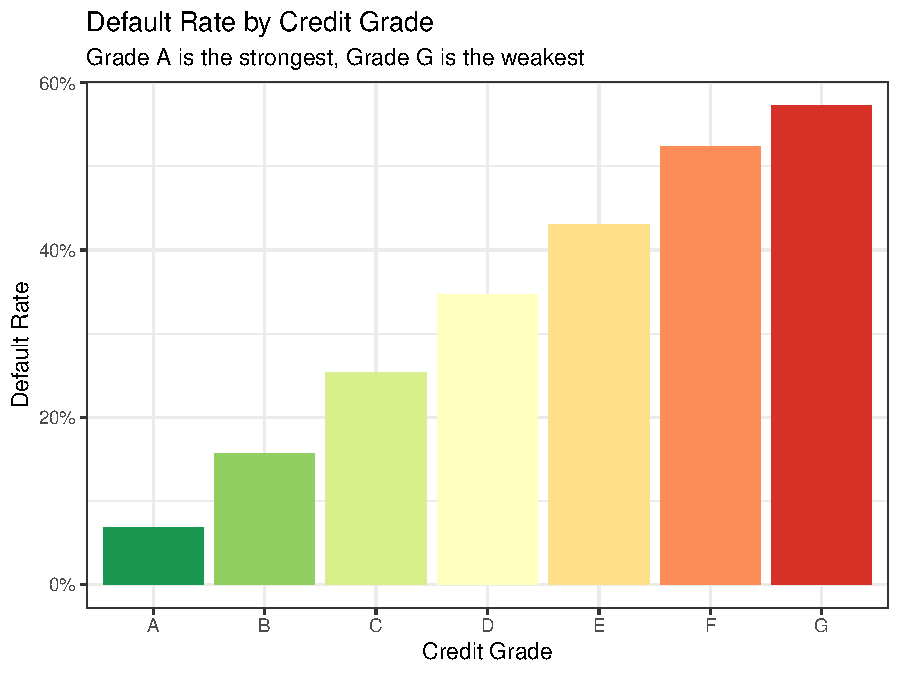
\includegraphics[keepaspectratio]{Question_3_files/figure-latex/unnamed-chunk-3-1.pdf}}

The Director's belief refers to grades A through F. The data also
contains a seventh grade, G, which was included here since it follows
the same pattern.

Credit grade predicts default very well. Default rates rise from 6.9\%
for Grade A to 57.3\% for Grade G, in a near perfectly increasing
staircase. This strongly supports the idea that grade is a great
indicator of default risk.

One part of the belief could not be tested. The data contains no age
column, so we cannot confirm whether grade is specifically a better or
worse predictor for younger individuals.

\pandocbounded{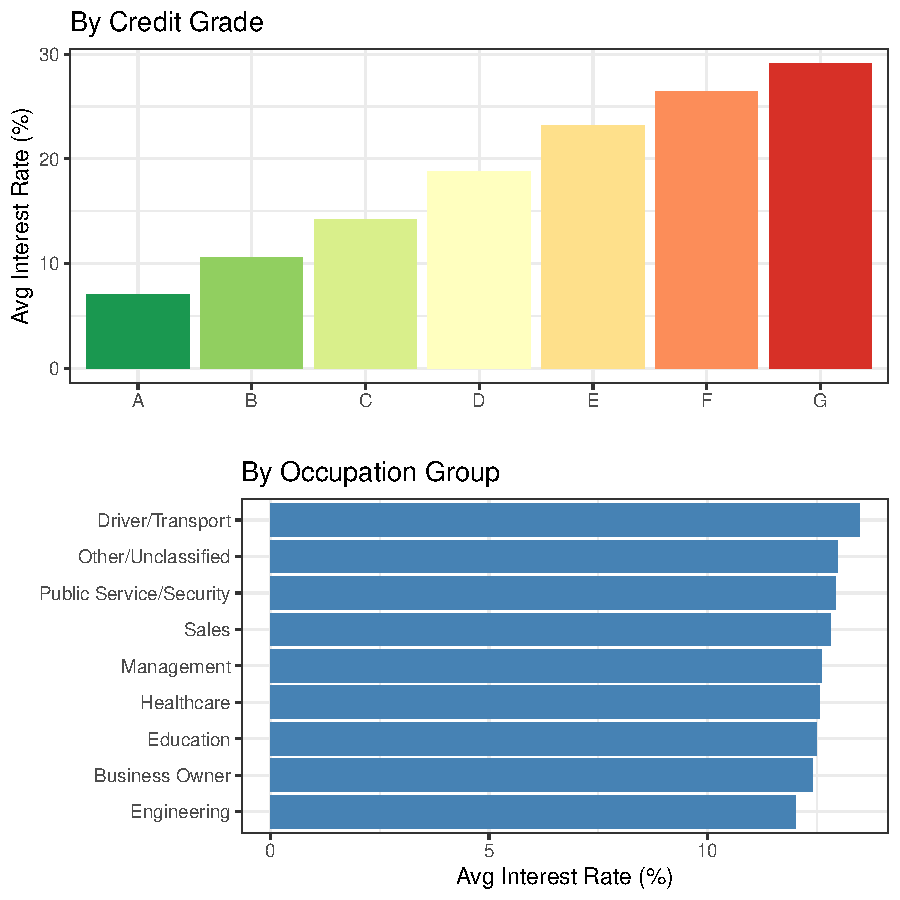
\includegraphics[keepaspectratio]{Question_3_files/figure-latex/unnamed-chunk-4-1.pdf}}

Credit grade strongly determines interest rate. Average rates rise from
7.0\% for Grade A to 29.1\% for Grade G, a spread of over 22 percentage
points.

Occupation has only a weak relationship with interest rate by
comparison. Average rates range from 12.0\% for Engineering to 13.5\%
for Driver/Transport, a spread of just 1.5 percentage points.

Occupation data required substantial cleaning before this comparison was
possible. Job titles were standardised for case and grouped into broad
categories using keyword matching. Even after this effort, 47\% of
records could not be confidently classified into a specific occupation
group and were kept as ``Other/Unclassified''. This limitation should be
kept in mind when interpreting the occupation comparison.

Taken together, the data suggests credit grade is by far the dominant
driver of interest rate. Occupation plays only a minor role. Age could
not be tested at all, since no age variable exists in this dataset.

\section{Debt-to-Income: Setting an Appropriate
Cap}\label{debt-to-income-setting-an-appropriate-cap}

\pandocbounded{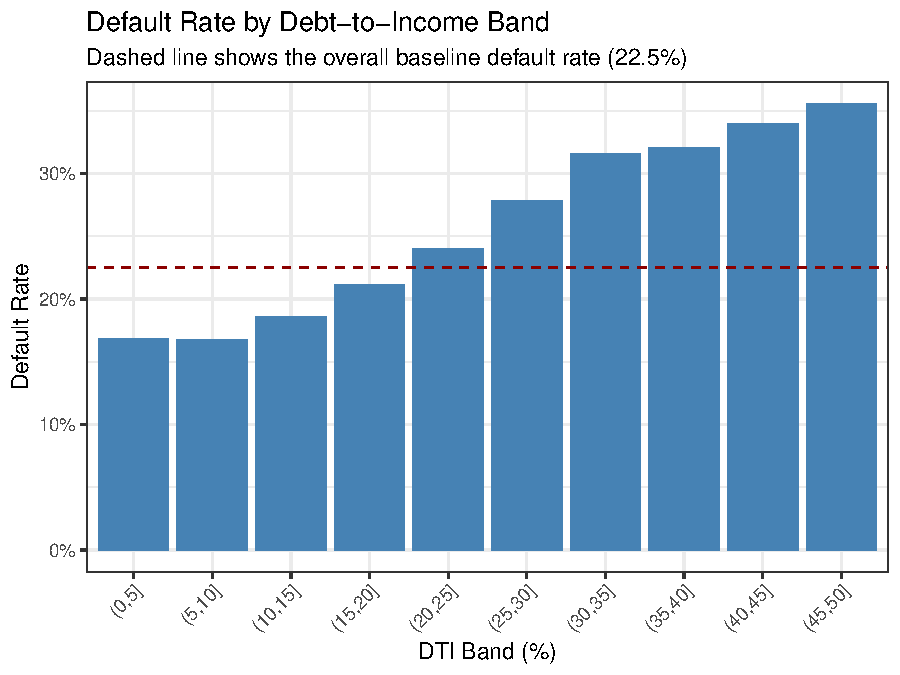
\includegraphics[keepaspectratio]{Question_3_files/figure-latex/unnamed-chunk-5-1.pdf}}

Default rate rises steadily and consistently with DTI. There is no
single point where risk suddenly jumps. This means the right DTI cap
depends on how much default risk the Institute is willing to accept,
rather than one universally correct number.

Loans with DTI up to 20\% default below the overall baseline rate of
22.5\%. Loans with DTI above 20\% cross into above-average risk
territory, and the gap widens steadily from there.

For a conservative risk tolerance, capping DTI at 20\% keeps default
rate at or below 21.2\%, modestly below the overall baseline.

For a moderate risk tolerance, capping DTI at 30\% allows a default rate
of around 27.9\%, still well below the riskiest bands.

For an aggressive risk tolerance, allowing DTI up to 40\% pushes default
rate to around 32.1\%, nearly 10 percentage points above baseline.

We would recommend a DTI cap in the region of 20\% to 25\% for most
lending purposes, balancing reasonable access to credit against
materially elevated default risk above this level.

The table below considers all loan terms, not only 36-month loans as in
the earlier state ranking. This is why the default rates shown here
differ slightly from those in the earlier section.

\begin{longtable}[]{@{}lrlr@{}}
\toprule\noalign{}
State & Avg DTI (\%) & Default Rate & N Loans \\
\midrule\noalign{}
\endhead
\bottomrule\noalign{}
\endlastfoot
AR & 20.3 & 27.5\% & 2849 \\
AL & 20.6 & 26.3\% & 4688 \\
TX & 19.5 & 22.8\% & 32277 \\
CA & 17.0 & 22.5\% & 53705 \\
VT & 20.7 & 15.3\% & 767 \\
ME & 19.8 & 14.4\% & 1256 \\
\end{longtable}

The relationship between DTI and default differs by state. Alabama's
average DTI (20.6\%) is actually higher than Maine's (19.8\%), yet
Alabama's default rate (26.3\%) is nearly double Maine's (14.4\%).

A single national DTI cap may not be equally appropriate everywhere. The
same DTI level appears to carry meaningfully different real-world
default risk depending on the state, echoing the broader state-level
differences found earlier in this report.

\section{Are the Institute's Heuristics
Realistic?}\label{are-the-institutes-heuristics-realistic}

Two of the three heuristics tested are well supported by the data. Home
ownership and employment length genuinely relate to default risk. States
genuinely differ in their default rates too.

The third heuristic is only partially realistic. Credit grade does
predict default very well, which supports part of the claim. The data
contains no age variable though, so the specific claim about younger
individuals could not be tested at all. The claim that interest rates
are clearly determined by occupation is also not well supported.
Occupation showed only a small relationship with interest rate,
especially compared to the much stronger relationship between credit
grade and interest rate.

The Institute's heuristics are mostly grounded in real patterns overall.
Some specific details, particularly around age and occupation, appear to
be assumptions rather than findings confirmed by this data.

\section{Summary and Recommendations}\label{summary-and-recommendations}

\textbf{Key risk drivers for default, in order of strength:}

\begin{itemize}
\tightlist
\item
  Credit grade is by far the strongest driver. Default rates rise from
  6.9\% for Grade A to 57.3\% for Grade G.
\item
  Debt-to-income ratio matters substantially too. Default rates rise
  steadily from around 17\% at low DTI to over 35\% at high DTI.
\item
  Home ownership status is a meaningful driver. Mortgage holders default
  least, renters default most.
\item
  Employment length adds further signal, particularly for mortgage
  holders and homeowners. Borrowers employed 10+ years default less
  often than those with shorter histories.
\item
  State of residence matters too, with default rates ranging from 10.6\%
  to 23.6\% across states, for reasons not fully explained by DTI alone.
\item
  Occupation, by contrast, shows only a weak relationship with
  risk-related outcomes once credit grade is accounted for.
\end{itemize}

\textbf{Customers most likely to default:}

The riskiest profile combines several of these factors at once: a low
credit grade, a high DTI, renting rather than owning, less than 10 years
in their current role, and residing in a higher-default state such as
Arkansas, Mississippi or Oklahoma. Each factor compounds the others, so
a borrower with several risk factors together is considerably riskier
than any single factor would suggest alone.

\textbf{What could reduce default risk in credibility assessment:}

\begin{itemize}
\tightlist
\item
  Continue relying heavily on credit grade, since it remains the
  strongest available predictor in this dataset.
\item
  Incorporate DTI more explicitly into assessment, given its steady and
  substantial relationship with default.
\item
  Consider state of residence as a contributing factor, given the
  meaningful spread found across states that DTI alone does not explain.
\item
  Treat occupation with caution as a standalone risk factor. The data
  does not support strong reliance on it once other factors are
  considered.
\item
  Collect age data going forward. Its complete absence from this dataset
  prevented testing an important part of the Institute's existing risk
  heuristics.
\end{itemize}

\bibliography{Tex/ref}





\end{document}
